\chapter{Analysis}
    After several consultations with the taxi company from the Mladá Boleslav we found out that in order to create such ordering system, our application must provide an interface to work with these five entities: Customers, Employees, Vehicles, Orders, and Notifications. 

In this chapter, we define each of these entities. We describe the data we want to store about them, the actions that can be performed with them and who is authorized to perform each of these actions. The overall goal of this chapter is to formalize the taxi company ordering process.
	
	
	\section{Customers}
		Customers are uniquely identified by telephone number. We also want to store about each of them this information:
		\begin{itemize}
			\item ID
			\item Name
			\item Note
			\item Fraud status
		\end{itemize}
	
		With Customer entity we are able to do these operations:
		\begin{itemize}
			\item Create and confirm
			\item Update
			\item Destroy
			\item Recover password
			\item Login and logout
			\item List favourite locations
			\item List all customers and show a specific customer
		\end{itemize}
		\subsection{Operation create and confirm}
			There are two ways of how the customer can be created. It is either directly through registration or indirectly by creating a new order.
			
			Directly registered customers are created in exchange for telephone number, password, and optional name. With this type of account customer can later login with a provided password. The application must verify the given telephone number.
			
			An indirectly registered user is created during the creation of a new order using a telephone number, which doesn't belong to any existing customer. This customer type is just an envelope with the purpose of information tracking and statistics - mostly for better customer support. This account type cannot be used for authentication. Indirectly registered user can be later registered directly with no difference to the normal direct registration.
		
		
		\subsection{Operation update}
			Customer can update only it's own name and password. Employees are able to change any customer's name, note, and fraud status.
		\subsection{Operation destroy}
            Destroying the customer can be invoked either by the customer itself or via the administrator. Orders made by that customer are not deleted - we just remove the information about the customer from the order.
		\subsection{Operation password recovery}
			In case of the lost password is a customer able to recover it. At first, the customer asks for the recovery with its telephone number. In return, it receives a recovery token via SMS. This token is valid for 5 minutes. In exchange for this token and the telephone number, the new password can be set. Customer is able to ask for the token resend. This will invalidate the last token, generate a new one and sends it via SMS.
		\subsection{Operation login and logout}
			With the login operation we receive login token in exchange for the telephone number and password. We send this token with each request to be authenticated.
			Customer can log in if and only if it is directly registered and confirmed.
			Logout just invalidates the session - customer must log in again to be authenticated.
		\subsection{Operation list favourite locations}
		    Our application must provide a list of customer favourite places. In the front-end applications is this operation called when the customer chooses its pick-up and drop-off location. 
		
		These places should be ordered with respect to the given location (current customer location or the selected pick-up location when choosing drop-off ). It should also take into account whether the customer chooses the pick-up or drop-off location. These recommendations should be based on the customer's order history and respect the start-finish relation of the orders. The most important are the first five places returned, so the place that the customer is most likely to choose based on current conditions should be amongst them. 
		
		Let's imagine a customer that has two routes - it often goes from pub to its home and sometimes goes from its home to the gym. In case of looking for the drop-off recommendation from unknown pick-up place, the application should return its home as the first item. When the user is asking for drop-off recommendation with pick-up at home, the application should return the gym as the first item, even though the pub is much more frequent place in its history.
		
		Only the user itself or the employees are able to see the favourite locations list.
		 
		\subsection{Operation list all customers and show specific customer}
            Our API must provide information about the customers created in our application.
			Show specific customer's data is available only for the customer itself or any employee. 
			
			List all the customers is available for the administrator only. The list of the customers is one of the most valuable taxi company's assets so we don't want to provide it for the staff. Of course that the employee could get all the customers by going one by one via operation show, but it takes more time so this is for our purpose enough.
		
	\section{Employees}
        There three types of employees - administrators, dispatchers and drivers. Employees, unlike customers, are identified via email. We store this information about each of them:
		\begin{itemize}
			\item Email
			\item Name
			\item Photograph
		\end{itemize}
		
		In our application, we have also the information about the employees' shifts - whether they are at work or not. For the drivers we also process current locations and their order queues. 
		
		Operations on employees are almost the same as operations on customers. Operations differ mainly in permissions. 
		\begin{itemize}
			\item Create and confirm
			\item Update
			\item Destroy
			\item Recover password
			\item Login and logout
			\item List all employees and show specific employee
		\end{itemize}
			\subsection{Operation create and confirm}
		An employee can be created by an administrator only. In exchange for the email, optional name, and image, the confirmation email is sent to the employee. Then the employee is redirected by clicking the link in email to the front-end page, where it sets its password. The link contains confirmation token which will the front-end application together with the optional name and image send to our application.
		
		\subsection{Operation update}		
		An employee can update its password, name and image. Besides these fields, an administrator can change the employee roles also.
		\subsection{Operation destroy}
		Only an administrator can remove an employee from the application. When the employee is removed, all the shifts and the driver queue is removed too. Orders associated with the employee remains in system but the corresponding employee field is removed.
		\subsection{Operation recover password}
        Recovering the forgotten password is exactly the same as in the customers' case - except the reset password token is hidden in a link sent via email.
		\subsection{Operation login and logout}
		The only difference between the employees and customers in these operations is that the employees log in with email instead of the telephone number. Everything else is the same.
		\subsection{Operation list all employees and show specific employee}
        Show all the employees or specific employee can only administrators and dispatchers. The rest (drivers, customers, anonymous users) can see only drivers who are on shift.

		There are also different attributes which are shown for different roles. Public attributes that anyone can see are id, name and image of the employee. Email, roles, and other attributes like creation and update timestamps are available to employee itself only, the dispatchers or the administrators.

		\subsection{Shifts}
			 Employees could be in three states: 
				\begin{itemize}
					\item available
					\item unavailable
					\item pause
				\end{itemize}
				Available means that the employee is on site and can handle orders. Unavailable is when it is not at work. Pause status is there for the situations when the employee knows that it won't be available for a while but wants to finish its orders.
				
				Switching directly from available to unavailable should be only in cases of emergency, e.g. driver has a flat tire and cannot continue. Employees will be instructed not to do so for better customer experience. 
				
				An employee is available to list the history of its shifts and administrator is available to list shifts for all the employees. Changing the shifts (available statuses) are employees allowed only for themselves.
		
		\subsection{Driver locations}
            Each driver sends since the shift start until the shift end its location in regular intervals. Driver's current location can be set only by the driver itself. See the driver's last available location can anyone, so the front-end can display the current location of arriving driver even for an anonymous customer. 
		
		\subsection{Driver order queues}
            Each driver has a queue of orders that are assigned to it. An administrator can see all the queues, a driver can see only its own queue.
	
	\section{Vehicles}
		Taxi company has the vehicle fleet we want to have in our system too. Each driver's shift starts with selecting the vehicle driver will ride in, so the customer can see and choose the car that fit its needs.
		
		 For each vehicle we have this information:
		\begin{itemize}
			\item name
			\item internal taxi company vehicle number used for communication
			\item plate
			\item image
			\item how many customers can fit in - required
			\item whether the vehicle is available for driving or not (e.g. is temporarily in the car repair shop)
		\end{itemize}
		These operations with vehicles our application supports:
		\begin{itemize}
			\item Create and update
			\item Show all and specific
			\item Destroy
		\end{itemize}
		\subsection{Operation create, update and destroy}
			Only administrators can create, update and destroy the company's vehicles. They can manipulate all the specified information. When the car is deleted, all the corresponding shifts or orders will have the vehicle value set to null.
		\subsection{Operation show all and specific vehicle}
			Administrators can see all the vehicles, others can see only the active ones. 
			Operations reveal all the attributes besides the internal vehicle number and the availability to anyone. Employees can see all of the attributes.
	\section{Orders}
	 	Order is a key entity in this application. Each order must go through the whole process from creation to successful finish or cancellation.
	 	
	 	There are two types of orders. The first one we call scheduled - a customer wants the taxi to arrive at the pick-up location at a specific date and time. In this type of order arriving at the specified time is crucial. The other type is when a customer just needs a taxi and sooner it arrives the better.
	 	
	 	Order is created from two sources - dispatchers and by customers directly.
	 	
	 	About each order we would like to keep this information:
		
		\begin{itemize}
			\item id
			\item status 
			\item driver who takes care of it
			\item vehicle by which it is processed with
			\item pick-up and drop-off location coordinates and addresses
			\item passenger count
			\item note
			\item contact telephone in case the customer is ordering for someone else
			\item estimated price
			\item whether the assigned driver cannot be changed (is explicitly chosen)
			\item VIP (just internal flag for the taxi company)
			\item flight number - in case the order is to/from the airport
			\item customer
			\item assigned dispatcher
			\item date and time the customer wants the taxi to arrive at the pick-up location (scheduled pick-up)
			\item source - whether it was created by dispatcher or directly by customer via front-end application
		\end{itemize}
		Also with the order we want to track these time parameters. In parenthesis is described how the time fields will be referenced in the whole thesis and the application:
		\begin{itemize}
			\item created time
			\item application estimate when the driver departs for a customer (start est.)
			\item when the driver started arriving to customer (start)
			\item estimation when will the driver arrive to the customer (arrived time est.)
			\item actual time when driver arrived to the customer - (arrived time)
			\item estimation and actual time when the driver has picked up  customer and starts driving to the drop-off destination (picked-up time est., picked-up time)
			\item finish time estimation and actual finished time(finish time, finish time est.)
		\end{itemize}
	
		Our goal is to have as much data about the order as possible, so we can later make statistics and analysis based on them. 
		
		These actions are needed for the orders module:
		\begin{itemize}
			\item show all / specific order
			\item list driver arrivals
			\item create order
			\item defraud and process
			\item confirm by driver
			\item refuse by driver
			\item arriving
			\item change arrive time
			\item arrived
			\item customer not on its place
			\item picked up
			\item change drop off time or location
			\item finished
			\item fraud
			\item my orders for dispatcher
			\item cancel
		\end{itemize}
		
		Because the order process is complex, we decided to sum it up in one illustration. This scheme displays all the order states (green), actions that can be done with the order and this application implements them (violet), time parameters we track (blue) and notifications which are sent in these actions (blue).
		
		\begin{figure}[H]
			\centering
			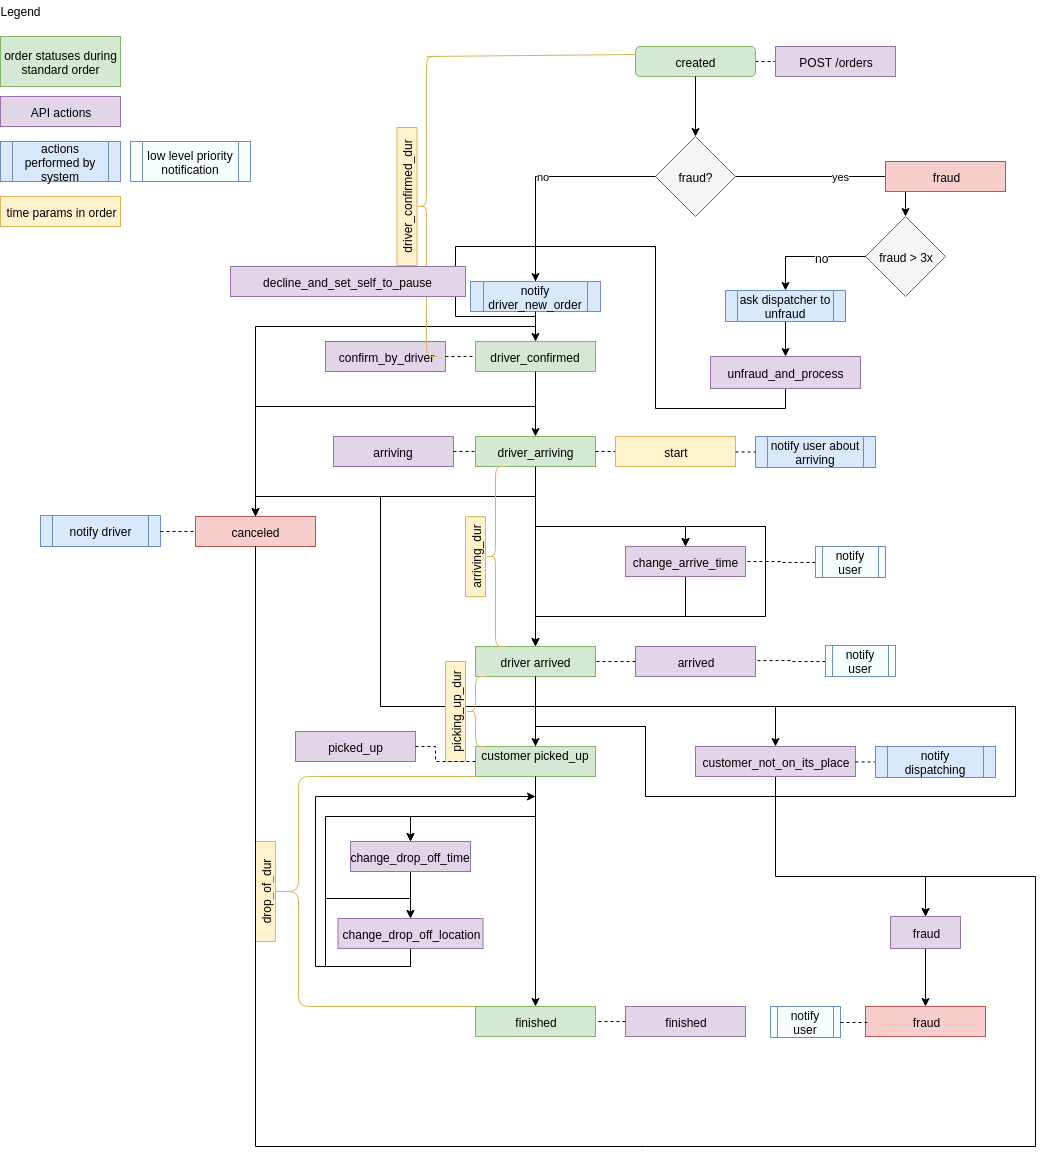
\includegraphics[width=\textwidth]{orders/order_process_scheme.png}
			\caption{Order process scheme}\label{order-process-scheme}
		\end{figure}
	
			In the next subsections, we describe in detail all the actions, their prerequisites, conditions, and outputs.
		
		\subsection{show all / specific order}
			Employees can see all the orders, customers can see only orders which they have made (even via dispatcher).
			
			We show specific attributes to the specific user types. Anyone (e.g. anonymous customers) can see order status, created time, arrived time est., finish time est.,  driver, and vehicle assigned to it. 
			
			A customer whose order it is can also see the coordinates and the addresses of start and finish, passenger count, note, contact telephone, estimated price, whether the assigned driver is selected explicitly, VIP flag, flight number, arrived time, scheduled pick up and source.
			
			Employees can besides all of the attributes above see the assigned dispatcher and all the tracked times, estimations and original estimations.
			
			Orders support basic filtering. We can get orders which are created since and until a specified time passed as parameter. We can retrieve also only scheduled orders. Orders can be filtered based on their status - we can set multiple statuses in which all the returned orders are.
			
			Orders are paginated - we can set via parameters which page to show and how much orders per page we retrieve.
			
			In a request for showing all the orders, we show the total order count for the specified query.
			
		\subsection{List driver arrivals}
		This action must return for the start and finish location list of the available drivers with their cars including the estimated arriving times for that location. This information then dispatcher tells the customer in case the order is via dispatching. In the other case, the customer can see it directly in the front-end application.
		
		This estimation doesn't have to be as precise as the estimation after the order is created.
		
		Same as in order creation it takes the driver parameter for the case that the customer wants the specific driver.
		
		This list is provided for anyone - even anonymous users.
		
		In case there is no driver available for such conditions it should return no available drivers result.
		\subsection{Create order}
			Order can be created in two ways. Either it is via dispatcher - customer calls the taxi company and the dispatcher will make the order or directly by customer via an app. 
			
			If the customer was marked as a fraud before, a new order is automatically marked as fraud one, thus it does not continue in the process and the creator is informed about that. If the fraud orders count in customer's history is less than three, one of the dispatchers on shift gets the notification whether this customer should be forgiven and the order can be processed. If the user has more than three fraud orders, dispatchers won't even get the notification about defrauding.
			
			Both the customer and dispatcher can explicitly choose a driver who takes care of the order. 
			
			Order will be assigned to the driver who can be at the pick-up location earliest. There is an exception for the scheduled orders - they are assigned to drivers exclusively by the dispatchers.
			
			If no driver is available for the specified parameters, it must return an error.
			
			After this action, order status is \textit{created}.
		\subsection{Defraud and process}
			This action is called by a dispatcher as a response to defraud notification - when it wants to forgive the customer frauds in history and wants to process the created order.
			
			If the customer is forgiven, it is marked as non-fraud and the order is processed as usual. From that moment on the customer is considered as a standard non-fraud user, so it can create subsequent orders without limitation. The forgiveness is though not definite - possible next fraud order will renew the original customer's fraud order count and increases the fraud count by one.
		\subsection{Confirm by driver}
			When an order is assigned to a driver, the driver confirms via this action the fact that it knows about it and is able to take it. Until this moment the arrive time estimation is very rough. This action can be performed only by the order's assigned driver and only if the order status is \textit{created}.
			
			This action changes the order status to \textit{driver\_confirmed}
		\subsection{Refuse by driver}
			A driver can also refuse an assigned order. We suppose that this will happen only in emergency cases. If the driver refuses the order, it is removed from its queue and passed on to the next available driver. If there's no one available the order is marked as cancelled.
			
			To refuse the order, its status must be \textit{created} and it can be done by the driver assigned to the order only.
		\subsection{Arriving}
			A driver can have more confirmed orders in its queue. When it starts to go to the customer, it calls the \textit{arriving} endpoint. This change the order status to \textit{driver\_arriving} and recalculate the time of arrival to the pick-up location. At this moment it should very precise estimation - the driver should be slowed down by the traffic only which is included in the Google Maps API. Thus at this moment, we send the SMS to the customer with the estimated time arrival.
			
			In order to call this action the order status must be \textit{driver\_confirmed} and it can be called by the driver assigned to order only. 
		\subsection{Change arrive time}
			A driver can correct the estimated arrival time based on its experience or unexpected complications during the journey.
			
			Correct the arrive time can the driver for his own orders only which are in the \textit{arriving} state.
		\subsection{Arrived}
			This request is sent when a driver arrives at the pick-up place. This changes the order status to \textit{arrived} and updates following times estimations because at this moment we know the real time of arrival.
			
			It can be set by the assigned driver only and only when the order status is \textit{arriving}.
		\subsection{Customer not on its place}
			In case the driver is at the pick-up location and cannot get in touch with the customer, this action is called. It sends the notification to the dispatching which takes care of the situation and communicates the problem between the driver and the customer. This situation can be resolved in two ways only. Either the customer is found and picked up, or it is not and the order is marked as fraud. 
			
			This action can be called when the order status is \textit{arrived} and by the driver assigned to the order only.
		\subsection{Picked up}
            In a point when the driver picks up the customer and is ready to ride to drop-off location this request is sent. Because now we know the picking up time precisely, drop off estimations can be recalculated. Also, this action changes the order status to \textit{customer\_picked\_up}.

			This action can be called only when order status is \textit{arrived} and only by driver whose the order is.
		\subsection{Change drop off time or location}
			Customers often don't know what they want, so in our application driver assigned to the order can change in this point the drop off time and also the location. This change leads to the recalculation of the estimated times. 
		\subsection{Finished}
		Order is marked by a driver as finished when he successfully handled whole order and is ready to serve another customer.
		\subsection{Fraud}
			Order can be marked as fraud from the \textit{driver\_arrived} and \textit{cancelled} order statuses. Mark order as fraud can the driver assigned to the order only. Marking the order as fraud resets the customer's fraud counter back to overall fraud orders count increased by one.
		\subsection{Cancel}
			Order can be cancelled by the driver assigned to order, dispatcher, or the customer whose order it is. In case the customer is anonymous it can be cancelled by anyone - because we cannot distinguish separate anonymous users.
			
			The only valid order statuses from which the order can be cancelled are \textit{'created'}, \textit{'driver\_confirmed'}, \textit{'driver\_arriving'} and \textit{'driver\_arrived'}.
			
		\subsection{My orders for dispatcher}
			Each order is assigned to a dispatcher. This dispatcher then takes care of the customers and in case of a problem must be able to react and handle it with the customer. For such purpose, there is this endpoint. A dispatcher can see all its orders with all important details such as the current time estimations, original estimations, customer number, assigned driver and so on.
			
			This endpoint shows only orders which are not finished, cancelled, or fraud, and the results are paginated.    
	
	\section{Notifications}
        Our system must have a way how to send messages to the users on specific actions. As described in the orders section, there are three types of notifications:
		\begin{itemize}
			\item driver has a new order
			\item customer is not at pick-up location
			\item new order from fraud customer
		\end{itemize}
		
		Each type contains specific data. \textit{Driver has new order} contains the order id. \textit{Customer not at pick-up location} contains driver id and name, customer id with telephone number. \textit{New order from fraud customer} contains order and customer id.
		
		
		Notification system is passive = front-end applications call our \textit{list notifications} action in regular intervals. User can mark the notification as resolved.
		
		
		\subsection{Operation list notifications}
			This operation returns all the notifications for the current user. The list is paginated via \textit{page} and \textit{per\_page} parameters. It also supports filtering only the unresolved notifications.
		\subsection{Operation mark as resolved}
			Notification can be marked as resolved only by the person to whom it belongs. 